\documentclass{standalone}
\usepackage{PhysicalChemistryNote}
\begin{document}
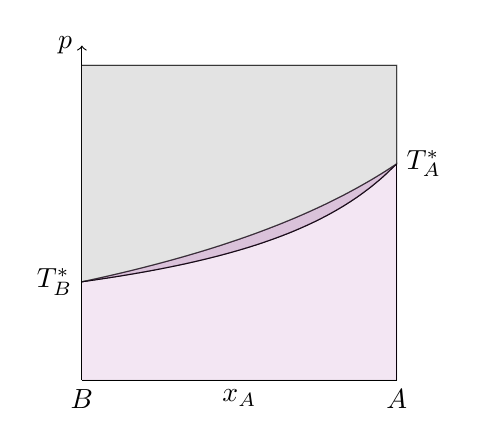
\begin{tikzpicture}
    \draw[-] (0,0) -- (4,0);
    \draw[->] (0,0) -- (0,4.25) node[left]{$p$};
    \draw[-] (4,0) -- (4,4);
    \draw[-] (0,4) -- (4,4);
    \node[below] at (0,0) {$B$};
    \node[below] at (4,0) {$A$};
    \node[below] at (2,0) {$x_{A}$};
    \draw[domain=0:4] plot[smooth](\x,{{-1/ln(-0.06145*(-7.3117-\x))}});
    \draw[domain=0:4] plot[smooth](\x,{1/ln(0.1967*(11.3117-\x))});
    \filldraw[fill=lightgray,opacity=0.25,domain=0:4] plot[smooth](\x,{-1/ln(-0.06145*(-7.3117-\x))}) -- (4,4) -- (0,4);
    \filldraw[fill=violet,opacity=0.05,domain=0:4] plot[smooth](\x,{-1/ln(-0.06145*(-7.3117-\x))}) -- (4,0) -- (0,0);
    \filldraw[fill=lightgray,opacity=0.25,domain=0:4] plot[smooth](\x,{1/ln(0.1967*(11.3117-\x))}) -- (4,4) -- (0,4);
    \filldraw[fill=violet,opacity=0.05,domain=0:4] plot[smooth](\x,{1/ln(0.1967*(11.3117-\x))}) -- (4,0) -- (0,0);
    \filldraw[fill=violet,opacity=0.15] plot[smooth,domain=0:4](\x,{{-1/ln(-0.06145*(-7.3117-\x))}})--plot[smooth,domain=4:0](\x,{1/ln(0.1967*(11.3117-\x))});
    \node[left] at (0,1.25) {$T_B^\ast$};
    \node[right] at (4,2.75) {$T_A^\ast$};
\end{tikzpicture}
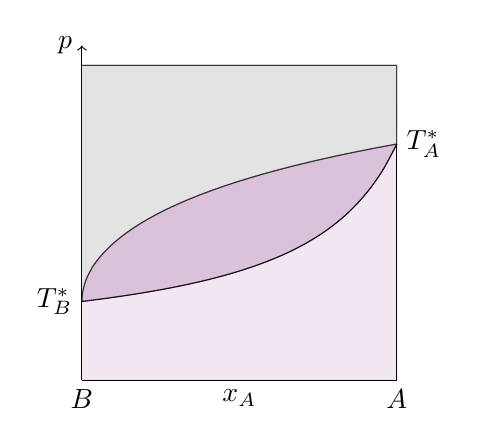
\begin{tikzpicture}
    \draw[-] (0,0) -- (4,0);
    \draw[->] (0,0) -- (0,4.25) node[left]{$p$};
    \draw[-] (4,0) -- (4,4);
    \draw[-] (0,4) -- (4,4);
    \node[below] at (0,0) {$B$};
    \node[below] at (4,0) {$A$};
    \node[below] at (2,0) {$x_{A}$};
    \draw[domain=0:4,samples=500] plot[smooth](\x,{(\x^0.5*(e^(-\x/6)/2+1))/1.2567+1});
    \draw[domain=0:4] plot[smooth](\x,{1/ln(0.25*(4*e+e^(1/3)*\x-e*\x))});
    \filldraw[fill=lightgray,opacity=0.25,domain=0:4,samples=500] plot[smooth](\x,{(\x^0.5*(e^(-\x/6)/2+1))/1.2567+1}) -- (4,4) -- (0,4);
    \filldraw[fill=violet,opacity=0.05,domain=0:4,samples=500] plot[smooth](\x,{(\x^0.5*(e^(-\x/6)/2+1))/1.2567+1}) -- (4,0) -- (0,0);
    \filldraw[fill=lightgray,opacity=0.25,domain=0:4] plot[smooth](\x,{1/ln(0.25*(4*e+e^(1/3)*\x-e*\x))}) -- (4,4) -- (0,4);
    \filldraw[fill=violet,opacity=0.05,domain=0:4] plot[smooth](\x,{1/ln(0.25*(4*e+e^(1/3)*\x-e*\x))}) -- (4,0) -- (0,0);
    \filldraw[fill=violet,opacity=0.15] plot[smooth,domain=0:4](\x,{1/ln(0.25*(4*e+e^(1/3)*\x-e*\x))}) -- plot[smooth,domain=4:0,samples=500](\x,{(\x^0.5*(e^(-\x/6)/2+1))/1.2567+1});
    \node[left] at (0,1) {$T_B^\ast$};
    \node[right] at (4,3) {$T_A^\ast$};
\end{tikzpicture}
\end{document}